%(BEGIN_QUESTION)
% Copyright 2006, Tony R. Kuphaldt, released under the Creative Commons Attribution License (v 1.0)
% This means you may do almost anything with this work of mine, so long as you give me proper credit

En fylt temperatursensor med indikator kalibreres i instrumentverkstedet med følerelementet (bulb) i samme høyde som bourdonrøret i indikatoren. I felt er imidlertid bulb montert betydelig høyere enn bourdonrøret.

$$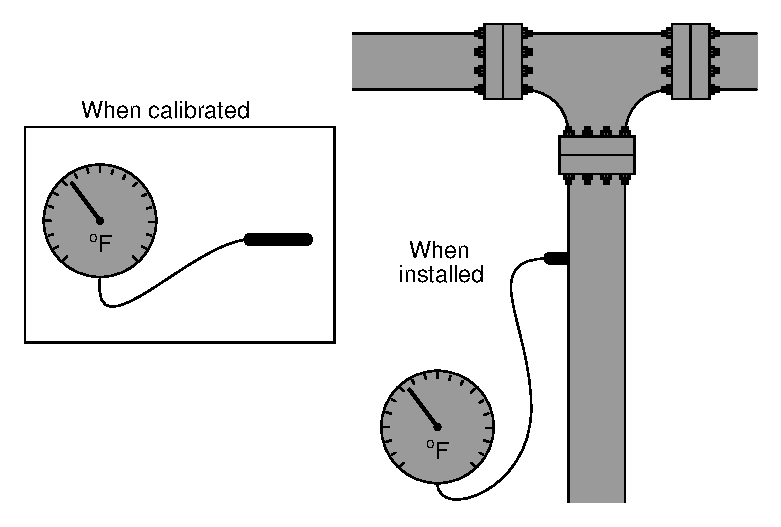
\includegraphics[width=15.5cm]{i00360x01.eps}$$

Vil dette gi målefeil? Hvis ja, hvilken type feil blir det (nullpunktskift eller spanskift)?

\vskip 20pt \vbox{\hrule \hbox{\strut \vrule{} {\bf Forslag til sokratisk diskusjon} \vrule} \hrule}

\begin{itemize}
\item{} Påvirkes alle klasser av fylte temperatursystemer likt av høydeforskjell?
\item{} Oppstår målefeil dersom instrumentet plasseres {\it over} bulb?
\item{} Hvordan ligner dette på utfordringer ved nivåmåling med hydrostatisk trykk? Finnes det et begrep vi bruker for dette?
\end{itemize}

\underbar{file i00360}
%(END_QUESTION)





%(BEGIN_ANSWER)

Høydeforskjell mellom bulb og indikatorelement påvirker bare noen klasser av fylte systemer, ikke alle. For disse systemene gir høydeforskjellen et nullpunktskift.

%(END_ANSWER)





%(BEGIN_NOTES)

Høydeforskjeller mellom bulb og indikatorelement påvirker bare fylte systemer der kapillarrøret inneholder væske. Dette omfatter Class I, Class IIA, Class IID og Class V. Class III påvirkes ikke av elevasjon eller suppresjon fordi arbeidsmediet er gass, og hydrostatisk trykk fra gassøylen blir neglisjerbart.

\vskip 10pt

I eksempelet vist her vil nullpunktet forskyves slik at indikatoren viser for høyt, på grunn av hydrostatisk trykk fra høydeforskjellen.

%INDEX% Measurement, temperature: filled-bulb system

%(END_NOTES)
